


\section{Méthode et outils}


De même que pour le développement du logiciel embarqué en \texttt{C++}, l'environnement de développement utilisé pour l'application web est \textit{Visual Studio Code}, associé à l'extension \textit{PlatformIO}. Cette combinaison permet de gérer efficacement le projet embarqué contenant le serveur web ainsi que le code exécuté sur le microcontrôleur ESP32.

Afin de faciliter le développement de l'interface utilisateur, un environnement serveur local est également utilisé. Celui-ci repose sur \textit{XAMPP}, qui fournit notamment un serveur \textit{Apache} permettant d'exécuter les fichiers constituant l'application web directement depuis l'ordinateur de développement.

L'utilisation de cet environnement local permet d'accélérer le cycle de développement. En effet, les modifications apportées aux fichiers HTML, CSS et JavaScript peuvent être testées instantanément dans un navigateur, sans nécessiter une nouvelle programmation (``flash'') de l'ESP32 après chaque changement. Cette approche simplifie le processus de débogage et permet de valider rapidement le comportement de l'interface avant son intégration dans le système embarqué.

Une fois les fonctionnalités de l'application validées, les fichiers nécessaires sont transférés dans la mémoire de l'ESP32 afin d'être utilisés par le serveur embarqué. Des tests finaux sont alors réalisés dans les conditions réelles d'utilisation afin de garantir le bon fonctionnement de l'ensemble du système.

\section{Architecture générale}

L'application développée repose sur une architecture client-serveur dans laquelle l'ESP32 joue le rôle de serveur embarqué. Celui-ci possède une interface WiFi permettant de créer un point d'accès auquel un client peut se connecter directement.

Après connexion au réseau WiFi généré par l'ESP32, l'utilisateur peut accéder au serveur web embarqué en utilisant l'adresse IP \texttt{192.168.4.1}. Cette adresse correspond à la passerelle du réseau créé par le microcontrôleur. Lorsqu'une requête est reçue, le serveur HTTP retourne les différents fichiers nécessaires au fonctionnement de l'application, notamment les pages HTML, les feuilles de style CSS ainsi que les scripts JavaScript.

Une fois l'interface web chargée dans le navigateur du client, une seconde communication est établie au moyen du protocole WebSocket. Contrairement au protocole HTTP classique basé sur un échange requête-réponse, WebSocket permet une communication bidirectionnelle permanente entre le client et l'ESP32. Ainsi, le navigateur peut transmettre des commandes au système embarqué, tandis que l'ESP32 peut envoyer spontanément des informations au client.

Cette architecture permet donc d'obtenir une interface réactive capable d'afficher l'état du système en temps réel tout en permettant à l'utilisateur d'interagir avec celui-ci.

\section{Serveur embarqué}

Le serveur embarqué est exécuté directement sur l'ESP32. Il assure deux fonctions principales : la distribution de l'application web au travers du protocole HTTP et l'échange de données en temps réel grâce au protocole WebSocket.

\subsection{Serveur \acrshort{http}}

Le serveur HTTP est responsable de la transmission des ressources nécessaires au fonctionnement de l'application web. Lorsqu'un utilisateur se connecte à l'adresse IP de l'ESP32, une requête HTTP est envoyée au microcontrôleur.

En réponse à cette requête, le serveur retourne les différents fichiers enregistrés dans sa mémoire, tels que les pages HTML, les fichiers CSS définissant l'apparence de l'interface ainsi que les scripts JavaScript assurant son fonctionnement dynamique.

L'utilisation d'un serveur HTTP directement intégré à l'ESP32 permet de supprimer la nécessité d'un serveur externe. L'ensemble de l'application peut ainsi fonctionner de manière autonome, uniquement avec le microcontrôleur et un appareil connecté au réseau WiFi.

\subsection{Serveur WebSocket}

Afin de permettre une communication en temps réel entre l'utilisateur et le système embarqué, un serveur WebSocket est utilisé en complément du serveur HTTP.

Contrairement au protocole HTTP, où chaque échange nécessite l'envoi d'une nouvelle requête, WebSocket maintient une connexion permanente entre le client et le serveur. Cette caractéristique permet aux deux parties d'envoyer des informations à tout moment.

Dans cette application, WebSocket est utilisé pour transmettre les commandes utilisateur vers l'ESP32, mais également pour retourner les informations provenant du système embarqué vers l'interface web. Cette communication bidirectionnelle permet notamment de mettre à jour l'affichage sans nécessiter de rafraîchissement manuel de la page.

\section{Application Web}


L'application web constitue l'interface entre l'utilisateur et le système embarqué. Elle est accessible depuis un navigateur web classique ou peut être installée sous la forme d'une application grâce à l'utilisation d'une Progressive Web App.

\subsection{Page Web}


L'application web est composée d'une unique page HTML principale. Cependant, cette dernière est organisée en plusieurs vues permettant de présenter à l'utilisateur différentes interfaces en fonction de la fonctionnalité sélectionnée. Cette technique correspond au principe d'une \textit{Single Page Application} (\acrshort{spa}).

Le principe d'une application monopage consiste à charger une seule fois la structure principale de l'application, puis à modifier dynamiquement son contenu à l'aide de scripts JavaScript, sans nécessiter le rechargement complet de la page. Ainsi, lors du passage d'une interface à une autre, seuls les éléments visibles sont modifiés tandis que la connexion avec le serveur reste active.

Cette approche présente plusieurs avantages dans le contexte de cette application. Elle permet notamment d'obtenir une navigation plus fluide, de réduire les échanges inutiles avec le serveur et de conserver la connexion WebSocket établie avec l'ESP32. Les différentes interfaces peuvent donc être affichées instantanément tout en continuant à recevoir les données envoyées par le système embarqué.
\subsubsection{Contrôle mouvement}

\begin{figure}[H]
    \centering
    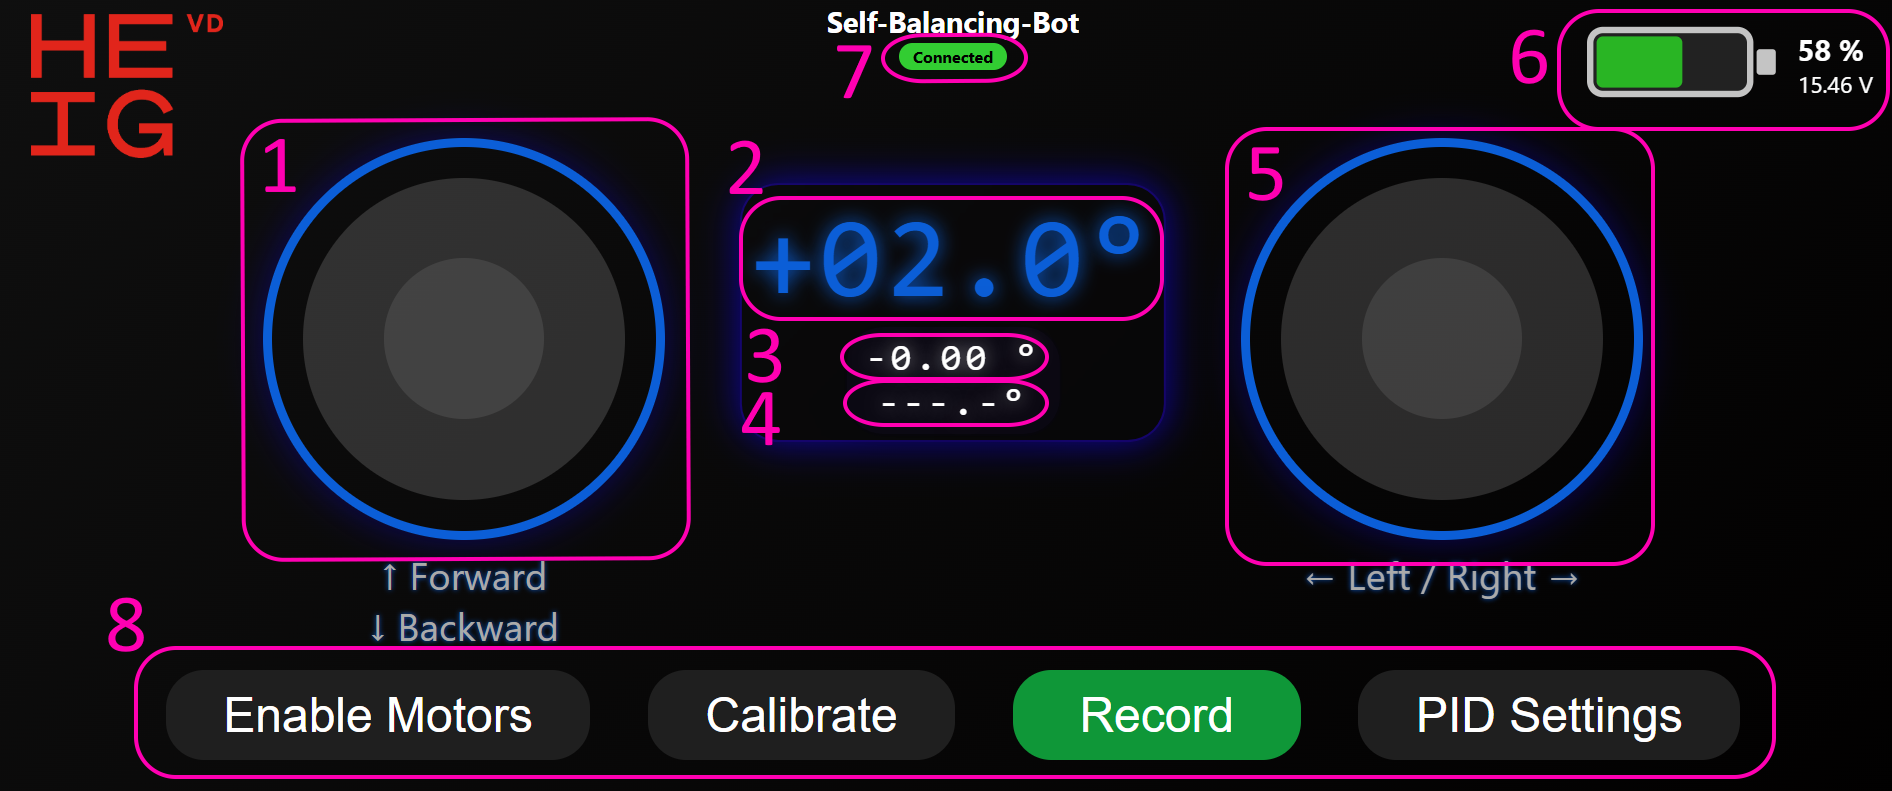
\includegraphics[width=1\textwidth]{assets/figures/UI1.png}
    \caption{Interface utilisateur pour le contrôle du mouvement}
    \label{fig:ui_mouvement}
\end{figure}
Cette vue permet à l'utilisateur d'interagir avec la partie déplacement du système.

\begin{table}[H]
\centering
\begin{tabularx}{\textwidth}{|l|X|}
\hline
\textbf{N°} & \textbf{Description} \\
\hline
1 & Joystick de contrôle de l'avance, recul.\\
\hline
2 & Angle $\theta$ instantané \\
\hline
3 & Angle d'équilibre (\texttt{theta\_offset}), peut être mis à jour par la pression du bouton \texttt{Calibrate} \\
\hline
4 & Consigne d'angle (\texttt{theta\_target}), donné par la boucle de régulation externe\\
\hline
5 & Joystick de contrôle rotation de l'angle $\psi$.\\
\hline
6 & Indicateur de batterie, mis à jour par le serveur périodiquement. \\
\hline
7 & Indicateur de connection WiFi et WebSocket. \\
\hline
8 & Boutons de contrôle \\
\hline
\end{tabularx}
\caption{Contrôle mouvement}
\end{table}

\begin{table}[H]
\centering
\begin{tabularx}{\textwidth}{|l|X|}
\hline
\textbf{Nom} & \textbf{Description} \\
\hline
\texttt{Enable Motors} & Active, désactive les moteurs, le texte du bouton change en fonction de l'état actuel des moteurs\\
\hline
\texttt{Calibrate} & Sauvegarde la valeur de l'angle actuel (\texttt{theta\_measured}) comme valeur d'angle d'équilibre (\texttt{theta\_offset}) \\
\hline
\texttt{Record} & Permet l'enregistrement des données, à la pression du bouton, l'enregistrement démarre, une seconde pression interromps l'enregistrement, les données sont transmises au client.\\
\hline
\texttt{PID Settings} & Accès à la seconde page de réglage des régulateurs \\
\hline
\end{tabularx}
\caption{Boutons de contrôle}
\end{table}

\subsubsection{Contrôle régulation}


\begin{figure}[H]
    \centering
    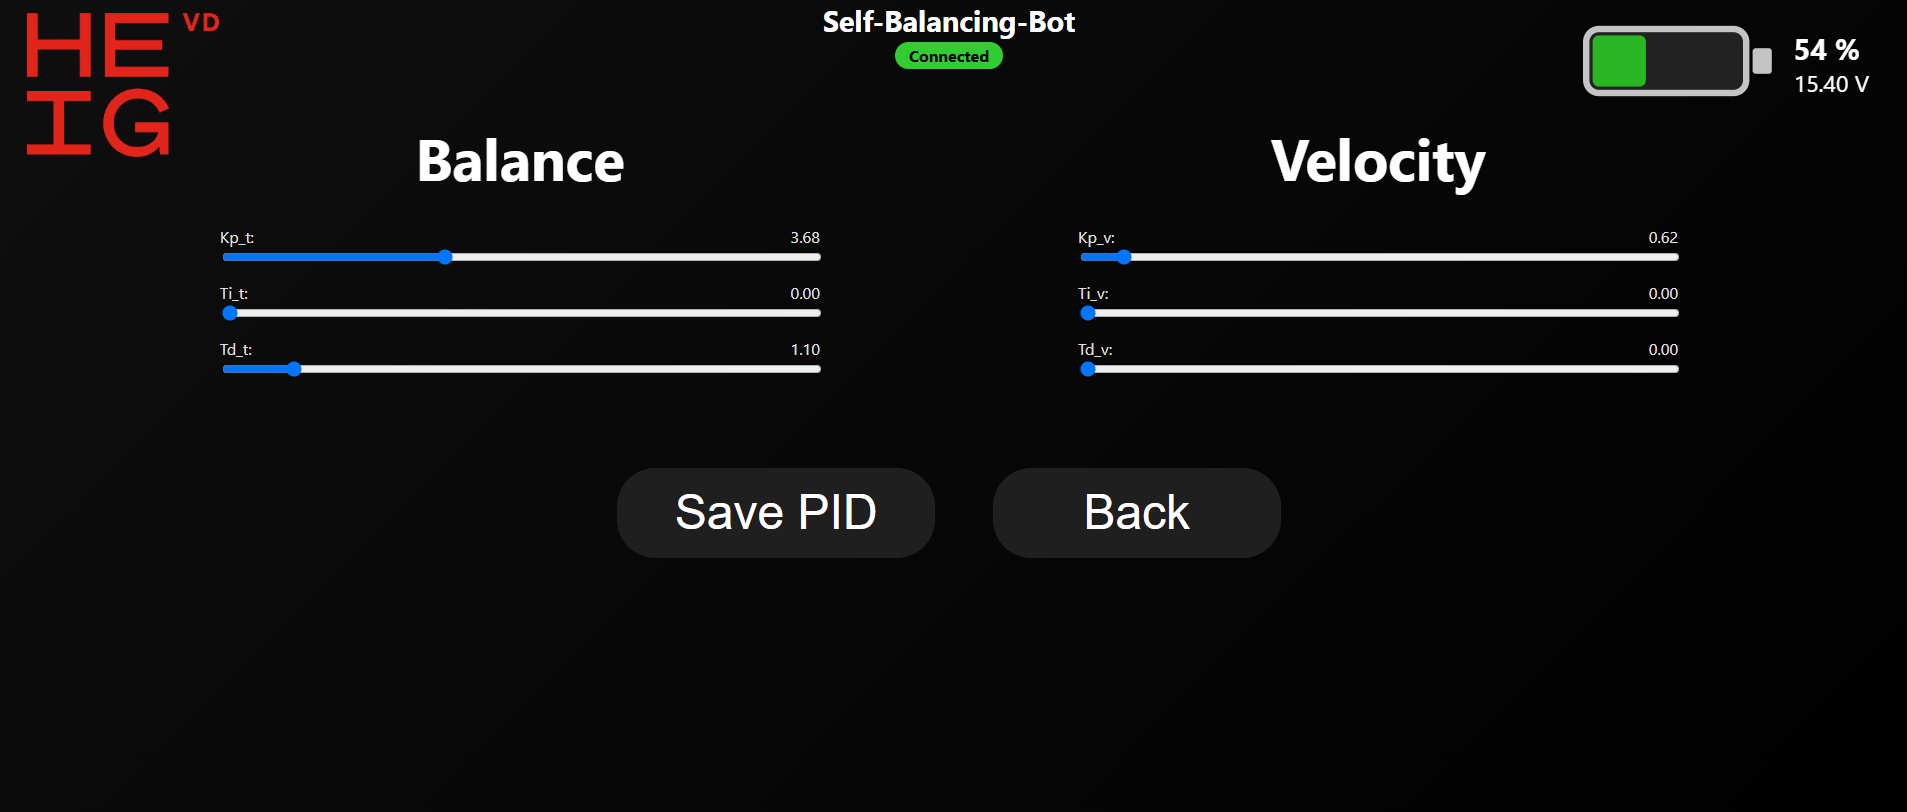
\includegraphics[width=1\textwidth]{assets/figures/UI2.png}
    \caption{Interface utilisateur pour le contrôle de la régulation}
    \label{fig:ui_regulation}
\end{figure}
Cette seconde vue permet à l'utilisateur de configurer les deux boucles de régulations indépendamment. A la pression du bouton \texttt{PID Settings}, une requête est envoyée au serveur, qui transmet alors les valeurs actuelles des régulateurs PID.

De cette manière, le client est toujours à jour lors des modifications effectuées.

Les données sont sauvées à la pression du bouton \texttt{Save PID}, cependant ces données sont perdues lors de la mise hors tension du système.

\subsection{PWA}

Afin d'améliorer l'expérience utilisateur, l'application web a été développée sous la forme d'une Progressive Web App (\acrshort{pwa}).

Une PWA est une application web pouvant être utilisée de manière similaire à une application native. Elle reste accessible depuis un navigateur mais peut également être installée directement sur un appareil compatible. Cette approche permet d'obtenir une interface plus proche d'une application mobile traditionnelle tout en conservant les avantages d'une application web.

L'utilisation d'une PWA permet notamment :
\begin{itemize}
    \item d'ajouter un raccourci vers l'application sur l'écran d'accueil ;
    \item d'utiliser une interface adaptée aux appareils mobiles ;
    \item de conserver une seule base de code pour différents types d'appareils ;
    \item de simplifier le déploiement de l'application.
\end{itemize}

L'implémentation repose sur un fichier \texttt{manifest.json} décrivant les informations générales de l'application, telles que son nom, ses icônes et son comportement lors du lancement.

\subsection{Installation}

L'installation de l'application est réalisée directement depuis un navigateur compatible. Lorsque les critères nécessaires sont remplis, celui-ci propose à l'utilisateur d'ajouter l'application à son appareil.

Une fois installée, la PWA apparaît comme une application classique et peut être lancée indépendamment du navigateur. L'utilisateur bénéficie ainsi d'un accès rapide à l'interface de contrôle de l'ESP32.
